\documentclass{article}
\usepackage{graphicx} % Required for inserting images

\title{proofs of Lemmas}
\author{Rohan Senapati}
\usepackage{url}
\usepackage{hyperref}
\usepackage{breakurl}
\usepackage{amssymb}
\usepackage{graphicx}
\usepackage[export]{adjustbox}
\usepackage[english]{babel}
\newtheorem{theorem}{Theorem}[section]
\newtheorem{corollary}{Corollary}[theorem]
\newtheorem{lemma}[theorem]{Lemma}
\newtheorem{conjecture}{Conjecture}
\newtheorem{definition}{Definition}
\date{July 2025}

\begin{document}

\maketitle

\section{Introduction}
\subsubsection{Rotational Symmetries}
In the rotational case, which is easier than the reflectional case, we can actually prove Lemma 7.3 directly. The first step of the rotational symmetry proofs is to assign $\omega$ to a $j-1^{th}$ root of unity. We then proceed to iterate $\omega$ over the polynomial $f(z) = z^j + c$. After a few iterations, we observe that each iterate rotates the previous one by $\omega$.
\\
\\
\textit{Proof of Lemma 7.3 Case 4}
\\
\\
$\underline{f(z) = z^4 + c}$           %Rotational Symmetries, f(z) = z^4 + c
\\
\\
Let $\omega$ = $e^{2\pi i/3}$
\\$f(z) = z^4+\omega c$
\\
\\$f(0) = 0^4 + \omega c = \omega c$
\\
\\$f(\omega c) = (\omega c)^4 + \omega c$
\\$\omega^3 = 1 \rightarrow \omega^4 = \omega$
\\$\rightarrow f(\omega c) = \omega c^4 + \omega c$
\\$= \omega(c^4+c)$
\\
\\$f(\omega(c^4+c)) = (\omega(c^4+c))^4 + \omega c$
\\$= \omega^4(c^4+c)^4 + \omega c$
\\$= \omega(c^4+c)^4 + \omega c$
\\$= \omega[(c^4+c)^4+c]$
\\
\\
\\
\textit{Proof of Lemma 7.3 Case 9}
\\
\\
$\underline{f(z) = z^5 + c}$          %Rotational Symmetries, f(z) = z^5 + c
\\
\\
Let $\omega$ = $e^{2\pi i/4}$
\\$\rightarrow\omega = i$
\\$f(z) = z^5+ic$
\\
\\$f(0) = 0^5 + ic = ic$
\\
\\$f(ic) = (ic)^5 + ic$
\\$i^4 = 1 \rightarrow i^5 = i$ or $\omega^4 = 1 \rightarrow\omega^5=\omega$
\\$(ic)^5 = i^5*c^5 = ic^5$
\\$\rightarrow f(ic) = ic^5 + ic$
\\$= i(c^5+c)$
\\
\\$f(i(c^5+c)) = (i(c^5+c))^5 +  ic$
\\$= i^5(c^5+c)^5 +  ic$
\\$= i(c^5+c)^5 + ic$
\\$= i[(c^5+c)^5+c]$
\\
\\
\\
\textit{Proof of Lemma 7.3 Case 11}
\\
\\
$\underline{f(z) = z^6 + c}$          %Rotational Symmetries, f(z) = z^6 + c
\\
\\
Let $\omega$ = $e^{2\pi i/5}$
\\$f(z) = z^6+\omega c$
\\
\\$f(0) = 0^6 + \omega c = \omega c$
\\
\\$f(\omega c) = (\omega c)^6 + \omega c$
\\$\omega^5 = 1 \rightarrow \omega^6 = \omega$
\\$\rightarrow f(\omega c) = \omega c^6 + \omega c$
\\$= \omega(c^6+c)$
\\
\\$f(\omega(c^6+c)) = (\omega(c^6+c))^6 + \omega c$
\\$= \omega^6(c^6+c)^6 + \omega c$
\\$= \omega(c^6+c)^6 + \omega c$
\\$= \omega[(c^6+c)^6+c]$
\\
\\Note : For rotations, Lemma 7.1 is immediately clear by taking absolute values.
\\
\\Disclaimer : After completing our work, we were informed that Cases 4, 9, and 11 of this lemma are also proved in the blog of Inigo Quilez [12], who is known for their beautiful mathematical visualizations.
\subsubsection{Reflectional Symmetries}
The next 16 cases regarding reflectional symmetry (from Lemmas 7.1 and 7.2) are proved by writing the formula for the reflection R in $(x, y)$ form. Using Wolfram Alpha, we checked some of the longer computations in this section.

\subsubsection{$f(z) = z^4 + c$}
\underline{$y=-\sqrt{3}x$}           %Reflectional Symmetries, f(z) = z^4 + c, y=-sqrt(3)x
\\
\\
\\$R(x,y) = (\frac{(1-(-\sqrt{3})^2)x+2(-\sqrt{3})y}{1+(-\sqrt{3})^2}, \frac{((-\sqrt{3})^2-1)y+2(-\sqrt{3})x}{1+(-\sqrt{3})^2})$
\\
\\$R(x,y) = (-\frac{1}{2}x-\frac{\sqrt{3}}{2}y, -\frac{\sqrt{3}}{2}x+\frac{1}{2}y)$
\\
\\\textit{Proof of Lemma 7.1 Case 1}
\\
\\Let $z=a+bi; (a,b)$
\\$R(z)$
\\$= R(a,b)$
\\$= (-\frac{1}{2}a-\frac{\sqrt{3}}{2}b, -\frac{\sqrt{3}}{2}a+\frac{1}{2}b)$
\\
\\$|R(z)|$
\\$= \sqrt{(-\frac{1}{2}a-\frac{\sqrt{3}}{2}b)^2 + (-\frac{\sqrt{3}}{2}a+\frac{1}{2}b)^2}$
\\$= \sqrt{a^2 + b^2}$
\\$= |z|$
\\
\\$|R(z)| = |z|$
\\
\\\textit{Proof of Lemma 7.2 Case 1}
\\
\\$z^4 = (a^4-6a^2b^2+b^4, 4a^3b-4ab^3)$
\\
\\$R(z^4)$
\\$= R(a^4-6a^2b^2+b^4, 4a^3b-4ab^3)$
\\$= (-\frac{1}{2}(a^4-6a^2b^2+b^4)-\frac{\sqrt{3}}{2}(4a^3b-4ab^3), -\frac{\sqrt{3}}{2}(a^4-6a^2b^2+b^4)+\frac{1}{2}(4a^3b-4ab^3))$
\\$= [-\frac{1}{2}(a^4-6a^2b^2+b^4)-\frac{\sqrt{3}}{2}(4a^3b-4ab^3)] + [-\frac{\sqrt{3}}{2}(a^4-6a^2b^2+b^4)+\frac{1}{2}(4a^3b-4ab^3))]i$
\\
\\$(R(z))^4$
\\$R(z)$
\\$= R(a,b)$
\\$= (-\frac{1}{2}a-\frac{\sqrt{3}}{2}b, -\frac{\sqrt{3}}{2}a+\frac{1}{2}b)$
\\$= [-\frac{1}{2}a-\frac{\sqrt{3}}{2}b] + [-\frac{\sqrt{3}}{2}a+\frac{1}{2}b]i$
\\$(R(z))^4$
\\$= ([-\frac{1}{2}a-\frac{\sqrt{3}}{2}b] + [-\frac{\sqrt{3}}{2}a+\frac{1}{2}b]i)^4$
\\$= [-\frac{1}{2}(a^4-6a^2b^2+b^4)-\frac{\sqrt{3}}{2}(4a^3b-4ab^3)] + [-\frac{\sqrt{3}}{2}(a^4-6a^2b^2+b^4)+\frac{1}{2}(4a^3b-4ab^3))]i$
\\$= R(z^4)$
\\
\\$R(z^4) = (R(z))^4$
\\
\\
\\
\\
\underline{$y=\sqrt{3}x$}           %Reflectional Symmetries, f(z) = z^4 + c, y=sqrt(3)x
\\
\\
$R(x,y) = (\frac{(1-(\sqrt{3})^2)x+2(\sqrt{3})y}{1+(\sqrt{3})^2}, \frac{((\sqrt{3})^2-1)y+2(\sqrt{3})x}{1+(\sqrt{3})^2})$
\\
\\$R(x,y) = (-\frac{1}{2}x+\frac{\sqrt{3}}{2}y, \frac{\sqrt{3}}{2}x+\frac{1}{2}y)$
\\
\\\textit{Proof of Lemma 7.1 Case 2}
\\
\\Let $z=a+bi; (a,b)$
\\$R(z)$
\\$= R(a,b)$
\\$= (-\frac{1}{2}a+\frac{\sqrt{3}}{2}b, \frac{\sqrt{3}}{2}a+\frac{1}{2}b)$
\\
\\$|R(z)|$
\\$= \sqrt{(-\frac{1}{2}a+\frac{\sqrt{3}}{2}b)^2 + (\frac{\sqrt{3}}{2}a+\frac{1}{2}b)^2}$
\\$= \sqrt{a^2 + b^2}$
\\$= |z|$
\\
\\$|R(z)| = |z|$
\\
\\\textit{Proof of Lemma 7.2 Case 2}
\\
\\$z^4 = (a+bi)^4 = a^4+4a^3bi-6a^2b^2-4ab^3i+b^4$
\\$= (a^4-6a^2b^2+b^4) + (4a^3b-4ab^3)i$
\\$= (a^4-6a^2b^2+b^4, 4a^3b-4ab^3)$
\\
\\$R(z^4)$
\\$= R(a^4-6a^2b^2+b^4, 4a^3b-4ab^3)$
\\$= (-\frac{1}{2}(a^4-6a^2b^2+b^4)+\frac{\sqrt{3}}{2}(4a^3b-4ab^3), \frac{\sqrt{3}}{2}(a^4-6a^2b^2+b^4)+\frac{1}{2}(4a^3b-4ab^3))$
\\$= [-\frac{1}{2}(a^4-6a^2b^2+b^4)+\frac{\sqrt{3}}{2}(4a^3b-4ab^3)] + [\frac{\sqrt{3}}{2}(a^4-6a^2b^2+b^4)+\frac{1}{2}(4a^3b-4ab^3))]i$
\\
\\$(R(z))^4$
\\$R(z)$
\\$= R(a,b)$
\\$= (-\frac{1}{2}a+\frac{\sqrt{3}}{2}b, \frac{\sqrt{3}}{2}a+\frac{1}{2}b)$
\\$= [-\frac{1}{2}a+\frac{\sqrt{3}}{2}b] + [\frac{\sqrt{3}}{2}a+\frac{1}{2}b]i$
\\$(R(z))^4$
\\$= ([-\frac{1}{2}a+\frac{\sqrt{3}}{2}b] + [\frac{\sqrt{3}}{2}a+\frac{1}{2}b]i)^4$
\\$= [-\frac{1}{2}(a^4-6a^2b^2+b^4)+\frac{\sqrt{3}}{2}(4a^3b-4ab^3)] + [\frac{\sqrt{3}}{2}(a^4-6a^2b^2+b^4)+\frac{1}{2}(4a^3b-4ab^3))]i$
\\$= R(z^4)$
\\
\\$R(z^4) = (R(z))^4$
\\
\\
\\
\\
\underline{$y=0$}           %Reflectional Symmetries, f(z) = z^4 + c, y=0
\\
\\
$R(x,y) = (\frac{(1-(0)^2)x+2(0)y}{1+(0)^2}, \frac{((0)^2-1)y+2(0)x}{1+(0)^2})$
\\
\\$R(x,y) = (x,-y)$
\\
\\\textit{Proof of Lemma 7.1 Case 3}
\\
\\Let $z=a+bi; (a,b)$
\\$R(z)= R(a,b)= (a,-b)$
\\
\\$|R(z)| = |(a,-b)|$
\\$= \sqrt{a^2+(-b)^2}$
\\$= \sqrt{a^2 + b^2}$
\\$= |z|$
\\
\\$|R(z)| = |z|$
\\
\\\textit{Proof of Lemma 7.2 Case 3}
\\
\\$z^4 = (a^4-6a^2b^2+b^4, 4a^3b-4ab^3)$
\\
\\$R(z^4)$
\\$= R(a^4-6a^2b^2+b^4, 4a^3b-4ab^3)$
\\$= (a^4-6a^2b^2+b^4, -[4a^3b-4ab^3])$
\\$= [a^4-6a^2b^2+b^4]+[-(4a^3b-4ab^3)]i$
\\
\\$(R(z))^4$
\\$= [a+(-b)i]^4$
\\$= [a^4-6a^2b^2+b^4]+[-(4a^3b-4ab^3)]i$
\\$= R(z^4)$
\\
\\$R(z^4) = (R(z))^4$
\\
\\
\subsubsection{$f(z) = z^5 + c$}
\underline{$y=x$}                %Reflectional Symmetries, f(z) = z^5 + c, y=x
\\
\\
$R(x,y) = (\frac{(1-(1)^2)x+2(1)y}{1+(1)^2}, \frac{((1)^2-1)y+2(1)x}{1+(1)^2})$
\\
\\$R(x,y) = (y, x)$
\\
\\\textit{Proof of Lemma 7.1 Case 5}
\\
\\Let $z=a+bi; (a,b)$
\\$R(z)$
\\$= R(a,b)$
\\$= (b, a)$
\\
\\$|R(z)|$
\\$=|(b,a)| $
\\$= \sqrt{b^2 + a^2}$
\\$= \sqrt{a^2 + b^2}$
\\$= |z|$
\\
\\$|R(z)| = |z|$
\\
\\\textit{Proof of Lemma 7.2 Case 5}
\\
\\$z^5 = (a+bi)^5$
\\$= a^5+5a^4bi-10a^3b^2-10a^2b^3i+5ab^4+b^5i$
\\$= a^5-10a^3b^2+5ab^4+5a^4bi-10a^2b^3i+b^5i$
\\$= [a^5-10a^3b^2+5ab^4]+[5a^4b-10a^2b^3+b^5]i$
\\$= (a^5-10a^3b^2+5ab^4, 5a^4b-10a^2b^3+b^5)$
\\
\\$R(z^5)$
\\$= R(a^5-10a^3b^2+5ab^4, 5a^4b-10a^2b^3+b^5)$
\\$= (5a^4b-10a^2b^3+b^5, a^5-10a^3b^2+5ab^4)$
\\$= [5a^4b-10a^2b^3+b^5] + [a^5-10a^3b^2+5ab^4]i$
\\
\\$(R(z))^5$
\\$= (b+ai)^5$
\\$= [5a^4b-10a^2b^3+b^5] + [a^5-10a^3b^2+5ab^4]i$
\\$= R(z^5)$
\\
\\$R(z^5) = (R(z))^5$
\\
\\
\\
\\
\underline{$y=0$}                %Reflectional Symmetries, f(z) = z^5 + c, y=0
\\
\\
$R(x,y) = (\frac{(1-(0)^2)x+2(0)y}{1+(0)^2}, \frac{((0)^2-1)y+2(0)x}{1+(0)^2})$
\\
\\$R(x,y) = (x, -y)$
\\
\\\textit{Proof of Lemma 7.1 Case 6}
\\
\\Let $z=a+bi; (a,b)$
\\$R(z)$
\\$= R(a,b)$
\\$= (a, -b)$
\\
\\$|R(z)|$
\\$=|(a,-b)| $
\\$= \sqrt{a^2 + (-b)^2}$
\\$= \sqrt{a^2 + b^2}$
\\$= |z|$
\\
\\$|R(z)| = |z|$
\\
\\\textit{Proof of Lemma 7.2 Case 6}
\\
\\$z^5 = (a^5-10a^3b^2+5ab^4, 5a^4b-10a^2b^3+b^5)$
\\
\\$R(z^5)$
\\$= R(a^5-10a^3b^2+5ab^4, 5a^4b-10a^2b^3+b^5)$
\\$= (a^5-10a^3b^2+5ab^4, -[5a^4b-10a^2b^3+b^5])$
\\$= [a^5-10a^3b^2+5ab^4] + (-[5a^4b-10a^2b^3+b^5])i$
\\
\\$(R(z))^5$
\\$= [a+(-b)i]^5$
\\$= [a^5-10a^3b^2+5ab^4] + (-[5a^4b-10a^2b^3+b^5])i$
\\$= R(z^5)$
\\
\\$R(z^5) = (R(z))^5$
\\
\\
\\
\\
\underline{$y=-x$}                %Reflectional Symmetries, f(z) = z^5 + c, y=-x
\\
\\
$R(x,y) = (\frac{(1-(-1)^2)x+2(-1)y}{1+(-1)^2}, \frac{((-1)^2-1)y+2(-1)x}{1+(-1)^2})$
\\
\\$R(x,y) = (-y, -x)$
\\
\\\textit{Proof of Lemma 7.1 Case 7}
\\
\\Let $z=a+bi; (a,b)$
\\$R(z)$
\\$= R(a,b)$
\\$= (-b, -a)$
\\
\\$|R(z)|$
\\$=|(-b,-a)| $
\\$= \sqrt{(-b)^2 + (-a)^2}$
\\$= \sqrt{a^2 + b^2}$
\\$= |z|$
\\
\\$|R(z)| = |z|$
\\
\\\textit{Proof of Lemma 7.2 Case 7}
\\
\\$z^5 = (a^5-10a^3b^2+5ab^4, 5a^4b-10a^2b^3+b^5)$
\\
\\$R(z^5)$
\\$= R(a^5-10a^3b^2+5ab^4, 5a^4b-10a^2b^3+b^5)$
\\$= (-[5a^4b-10a^2b^3+b^5], -[a^5-10a^3b^2+5ab^4])$
\\$= -[5a^4b-10a^2b^3+b^5] + (-[a^5-10a^3b^2+5ab^4])i$
\\
\\$(R(z))^5$
\\$= [(-b)+(-a)i]^5$
\\$= -[5a^4b-10a^2b^3+b^5] + (-[a^5-10a^3b^2+5ab^4])i$
\\$= R(z^5)$
\\
\\$R(z^5) = (R(z))^5$
\\
\\
\\
\\
\underline{$x=0$}                %Reflectional Symmetries, f(z) = z^5 + c, x=0
\\
\\
$R(x,y)$
\\$= \lim_{x \to \infty} (\frac{(1-(m)^2)x+2(m)y}{1+(m)^2}, \frac{((m)^2-1)y+2(m)x}{1+(m)^2})$
\\$= \lim_{x \to \infty} (\frac{(-(m)^2)x+2(m)y}{(m)^2}, \frac{((m)^2)y+2(m)x}{(m)^2})$
\\$= \lim_{x \to \infty} (-x+\frac{2y}{m}, y+\frac{2x}{m})$
\\$= (-x,y)$
\\
\\$R(x,y) = (-x, y)$
\\
\\\textit{Proof of Lemma 7.1 Case 8}
\\
\\Let $z=a+bi; (a,b)$
\\$R(z)$
\\$= R(a,b)$
\\$= (-a, b)$
\\
\\$|R(z)|$
\\$=|(-a,b)| $
\\$= \sqrt{(-a)^2 + (b)^2}$
\\$= \sqrt{a^2 + b^2}$
\\$= |z|$
\\
\\$|R(z)| = |z|$
\\
\\\textit{Proof of Lemma 7.2 Case 8}
\\
\\$z^5 = (a^5-10a^3b^2+5ab^4, 5a^4b-10a^2b^3+b^5)$
\\
\\$R(z^5)$
\\$= R(a^5-10a^3b^2+5ab^4, 5a^4b-10a^2b^3+b^5)$
\\$= (-[a^5-10a^3b^2+5ab^4], 5a^4b-10a^2b^3+b^5)$
\\$= -[a^5-10a^3b^2+5ab^4] + [5a^4b-10a^2b^3+b^5]i$
\\
\\$(R(z))^5$
\\$= (-a+bi)^5$
\\$= -[a^5-10a^3b^2+5ab^4] + [5a^4b-10a^2b^3+b^5]i$
\\$= R(z^5)$
\\
\\$R(z^5) = (R(z))^5$
\\
\\
\\
\\
\subsubsection{$f(z) = z^6 + c$}
\underline{$f(z) = z^6 + c, y=\tan(\frac{2\pi}{5})x$}
\\
\\
$R(x,y) = (\frac{[(1-\tan^2(\frac{2\pi}{5})]x+2\tan(\frac{2\pi}{5})y}{1+\tan^2(\frac{2\pi}{5})}, \frac{[\tan^2(\frac{2\pi}{5})-1]y+2\tan(\frac{2\pi}{5})x}{1+\tan^2(\frac{2\pi}{5})})$
\\$= (\frac{[(1-\tan^2(\frac{2\pi}{5})]x+2\tan(\frac{2\pi}{5})y}{\sec^2(\frac{2\pi}{5})}, \frac{[\tan^2(\frac{2\pi}{5})-1]y+2\tan(\frac{2\pi}{5})x}{\sec^2(\frac{2\pi}{5})})$
\\
\\
\\\textit{Proof of Lemma 7.1 Case 10}
\\
\\Let $z=a+bi; (a,b)$
\\$|R(z)|$
\\$= |R(a,b)|$
\\$=|(\frac{[(1-\tan^2(\frac{2\pi}{5})]a+2\tan(\frac{2\pi}{5})b}{\sec^2(\frac{2\pi}{5})},\frac{[\tan^2(\frac{2\pi}{5})-1]b+2\tan(\frac{2\pi}{5})a}{\sec^2(\frac{2\pi}{5})})|$
\\$\sqrt{(\frac{[(1-\tan^2(\frac{2\pi}{5})]a+2\tan(\frac{2\pi}{5})b}{\sec^2(\frac{2\pi}{5})})^2+(\frac{[\tan^2(\frac{2\pi}{5})-1]b+2\tan(\frac{2\pi}{5})a}{\sec^2(\frac{2\pi}{5})})^2}$
\\$= \sqrt{a^2+b^2}$
\\$= |z|$
\\
\\$|R(z)| = |z|$
\\
\\\textit{Proof of Lemma 7.2 Case 10}
\\
\\$z^6 = (a+bi)^6$
\\$= a^6+6a^5bi-15a^4b^2-20a^3b^3i+15a^2b^4+6ab^5i-b^6$
\\$= a^6-15a^4b^2+15a^2b^4-b^6+6a^5bi-20a^3b^3i+6ab^5i$
\\$= [a^6-15a^4b^2+15a^2b^4-b^6]+[6a^5b-20a^3b^3+6ab^5]i$
\\$= (a^6-15a^4b^2+15a^2b^4-b^6, 6a^5b-20a^3b^3+6ab^5)$
\\
\\$R(z^6)$
\\$= R(a^6-15a^4b^2+15a^2b^4-b^6, 6a^5b-20a^3b^3+6ab^5)$
\\$= (\frac{[(1-\tan^2(\frac{2\pi}{5})](a^6-15a^4b^2+15a^2b^4-b^6)+2\tan(\frac{2\pi}{5})(6a^5b-20a^3b^3+6ab^5)}{\sec^2(\frac{2\pi}{5})}$, 
\\$\frac{[\tan^2(\frac{2\pi}{5})-1](6a^5b-20a^3b^3+6ab^5)+2\tan(\frac{2\pi}{5})(a^6-15a^4b^2+15a^2b^4-b^6)}{\sec^2(\frac{2\pi}{5})})$
\\$= \frac{[(1-\tan^2(\frac{2\pi}{5})](a^6-15a^4b^2+15a^2b^4-b^6)+2\tan(\frac{2\pi}{5})(6a^5b-20a^3b^3+6ab^5)}{\sec^2(\frac{2\pi}{5})}$
\\$+ \frac{[\tan^2(\frac{2\pi}{5})-1](6a^5b-20a^3b^3+6ab^5)+2\tan(\frac{2\pi}{5})(a^6-15a^4b^2+15a^2b^4-b^6)}{\sec^2(\frac{2\pi}{5})}i$
\\
\\$(R(z))^6$
\\$=(\frac{[(1-\tan^2(\frac{2\pi}{5})]a+2\tan(\frac{2\pi}{5})b}{\sec^2(\frac{2\pi}{5})}+\frac{[\tan^2(\frac{2\pi}{5})-1]b+2\tan(\frac{2\pi}{5})a}{\sec^2(\frac{2\pi}{5})}i)^6$
\\$= \frac{[(1-\tan^2(\frac{2\pi}{5})](a^6-15a^4b^2+15a^2b^4-b^6)+2\tan(\frac{2\pi}{5})(6a^5b-20a^3b^3+6ab^5)}{\sec^2(\frac{2\pi}{5})}$
\\$+ \frac{[\tan^2(\frac{2\pi}{5})-1](6a^5b-20a^3b^3+6ab^5)+2\tan(\frac{2\pi}{5})(a^6-15a^4b^2+15a^2b^4-b^6)}{\sec^2(\frac{2\pi}{5})}i$
\\$= R(z^6)$
\\
\\$R(z^6) = (R(z))^6$
\\
\\While equality may not seem immediately obvious due to its large computational nature, the corresponding contour plots of $R(z)^6$ and $(R(z))^6$ match, strongly suggesting equality.
\\
\\
\\
\begin{minipage}{0.6\textwidth}
    \centering
    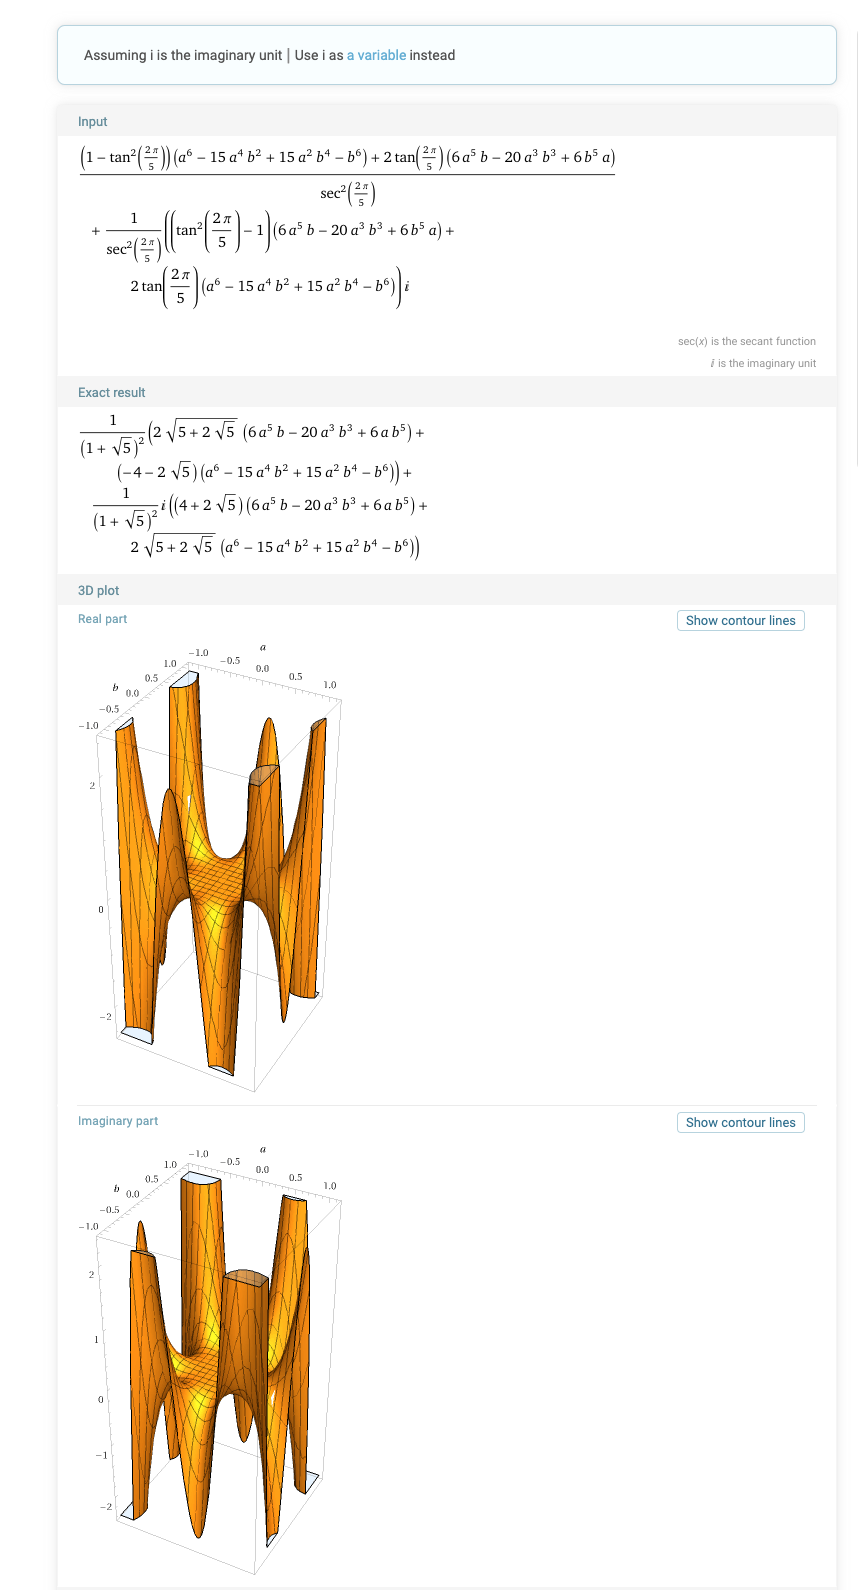
\includegraphics[width=0.9\textwidth]{R(z)^6.png}
    \caption{$R(z)^6$}
\end{minipage}%
\begin{minipage}{0.6\textwidth}
    \centering
    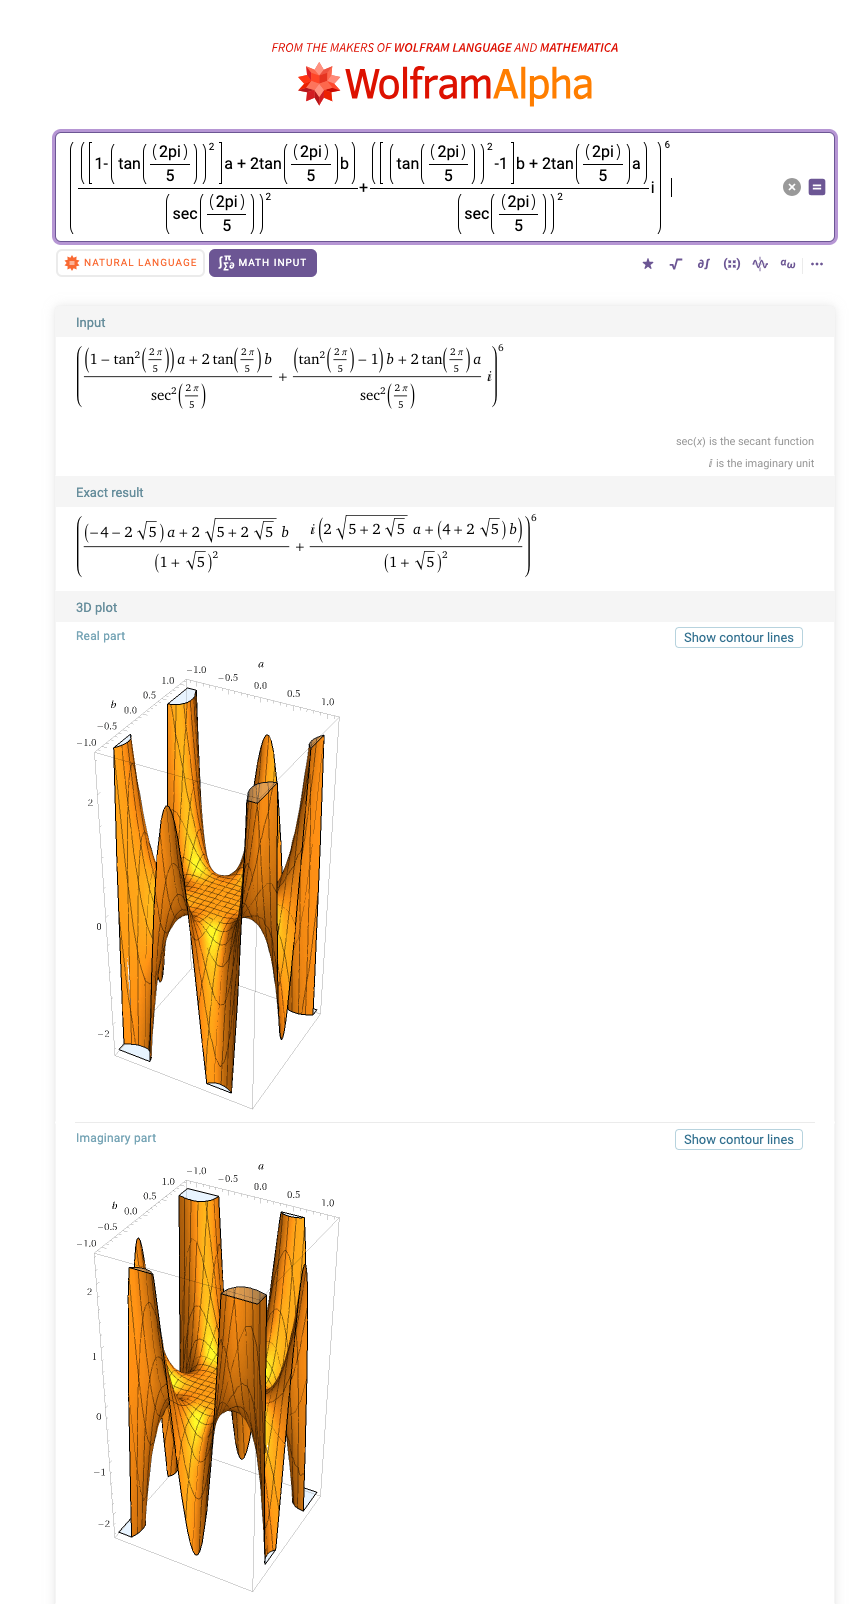
\includegraphics[width=0.9\textwidth]{(R(z))^6.png}
    \caption{$(R(z))^6$}
\end{minipage}

\end{document}